
%----------------------------------------------------------------------------------------
%	Lecture 4
%----------------------------------------------------------------------------------------

\chapter{Min-Max Problems}

\bigbreak
\section{Local Maxima or Minima}

At a local maxima and minima, $f_x = 0$ and $f_y = 0$ are both zero at the same time.
We can proof this by contradiction. 
If $f_x$ or $f_y$ were non-zero then we can increase of decrease the value of $x$ or $y$ respectively
to get a higher or lower value depending on whether the point is maxima or minima.

The approximation formula tells us that if both partial derivatives are zero then the height of the graph does not change, 
which means that the tangent plant to the graph is horizontal.

{\bf Critical Point : } $(x_0, y_0)$ is a critical point if $f_x(x_0, y_0) = 0$ and $f_y(x_0, y_0) = 0$.
In general, if a function depeneds on many variables then a critical point is the point at which all the partial derivatives of that function are zero.

In single variable functions, the critical points are either minima or maxima.
But here there is another kind of point. Its called a Saddle Point. 
It occurs when the function value is minima in one direction and maxima in the other dimention.

\begin{figure}[ht!]
    \centering
    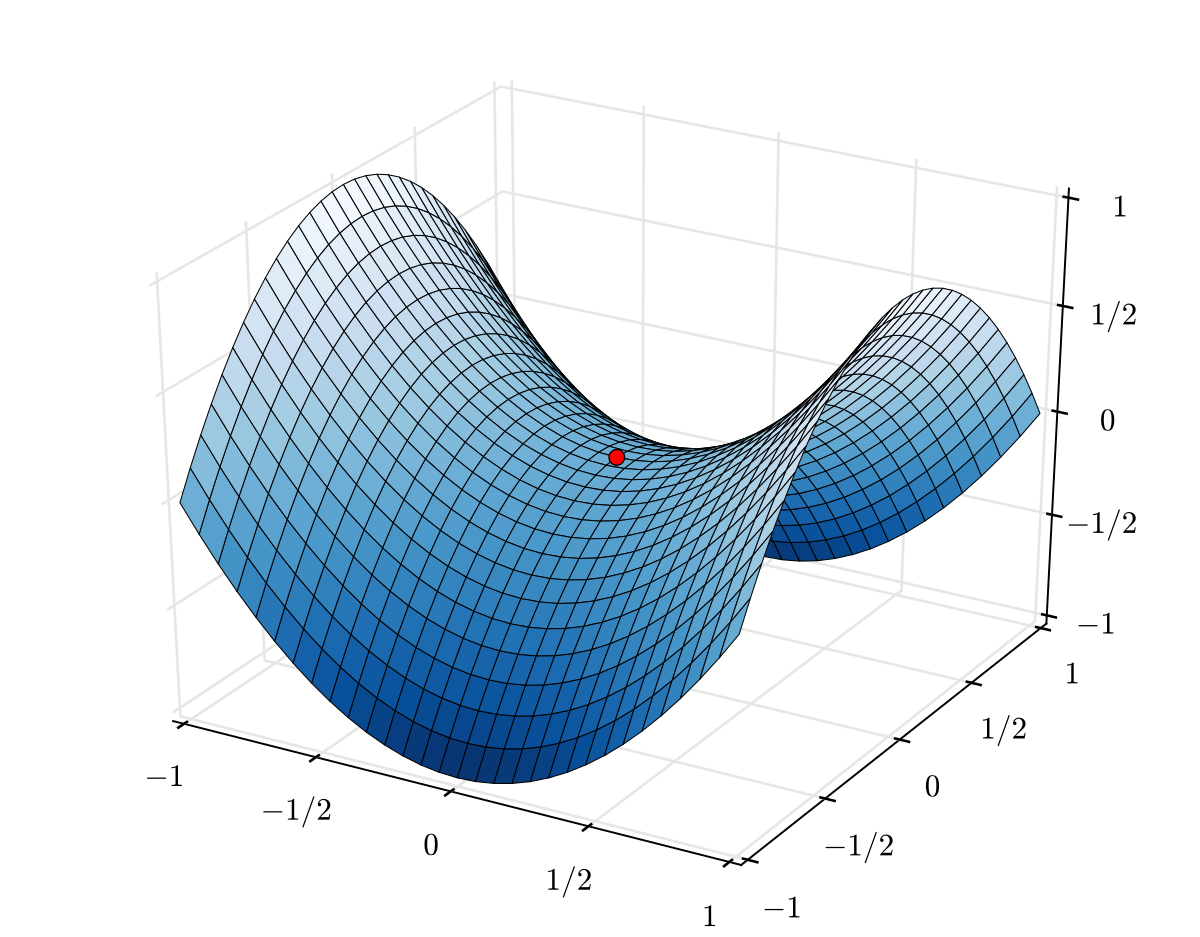
\includegraphics[scale=0.25]{./images/lecture_4_figure_1.png}
    \caption{Saddle Point}
\end{figure}

Here you can see that if we slice across one plane then it is a minima.
But if we slice across the other plane then it is a maxima. 
Thus, it is neither a local maxima or minima.
